%--------------------
% Packages
% -------------------
\documentclass[11pt,a4paper]{article}
\usepackage[utf8x]{inputenc}
\usepackage[T1]{fontenc}
%\usepackage{gentium}
\usepackage{mathptmx} % Use Times Font
% \usepackage{wordcount}


\usepackage[pdftex]{graphicx} % Required for including pictures
\usepackage[pdftex,linkcolor=black,pdfborder={0 0 0}]{hyperref} % Format links for pdf
\usepackage{calc} % To reset the counter in the document after title page
\usepackage[numbers]{natbib}


\frenchspacing % No double spacing between sentences
\linespread{1.2} % Set linespace
\usepackage[a4paper, lmargin=0.1666\paperwidth, rmargin=0.1666\paperwidth, tmargin=0.1111\paperheight, bmargin=0.1111\paperheight]{geometry} %margins
%\usepackage{parskip}

\usepackage[all]{nowidow} % Tries to remove widows
\usepackage[protrusion=true,expansion=true]{microtype} % Improves typography, load after fontpackage is selected


%-----------------------
% Set pdf information and add title, fill in the fields
%-----------------------
\hypersetup{ 	
pdfsubject = {Machine Learning Coursework},
pdftitle = {Machine Learning Coursework},
pdfauthor = {Laura Just Fung (lj441)}
}

%-----------------------
% Begin document
%-----------------------
\begin{document} 

\begin{center}
    \LARGE{\textbf{Machine Learning Coursework Assignment}}
    \\
    \Large{{Adding two MNIST digits through an inference pipeline}}
    \\
    \large{Laura Just Fung (lj441)}
    \\
    \today
    \\
    Word count: 2994
\end{center}

\section{Introduction}

MNIST is a dataset consisting of handwritten digits and their labels commonly used for training machine learning models and image processing systems \citep{deng2012mnist}. The classical problem represented by the MNIST dataset is for machine learning algorithms to be able to learn to recognise handwritten digits, no matter how they are shaped.

For this project, the problem at hand is not just for the inference pipeline to learn to recognise MNIST digits accurately, it must also learn addition.

First, a stratified dataset of paired MNIST digits will be generated, along with the label denoting their sum. Then, a neural network will be trained and perform supervised learning on this dataset. Hyperparameter tuning will be performed using \texttt{Optuna}.

To explore this problem further, a SVM, a random forest, and an AdaBoost classifier were also trained on the MNIST dataset. Weak linear classifiers were also used.

The t-SNE distribution of the dataset and the embedding layer of the best-performing neural network were also extracted and analysed, optimising for perplexity.

\section{Dataset generation}
The dataset upon which the models were trained on was first loaded in from MNIST using \texttt{Tensorflow}. For datasets greater than and divisible by 100, stratified data sampling was used, such that each permutation of digit pairs was represented equally. For datasets less than 100 samples in size, each pair was randomly picked from a list of all possible permutations without replacement.

For larger datasets, equal representation of the pairs was judged to be more important than sampling without replacement from the MNIST dataset. The risk of data leakage and the models learning from the handwriting shapes rather than the numbers was judged to be minimal, as the training and validation/testing data were drawn from separate parts of the MNIST dataset. This was achieved by splitting the MNIST dataset when it was first loaded and then constructing the training and validation/testing datasets from each subset separately. The results of these samplings can be found in Fig.~\ref{fig:manysamples} and Fig.~\ref{fig:fewsamples} respectively.

\begin{figure}
    \centering
    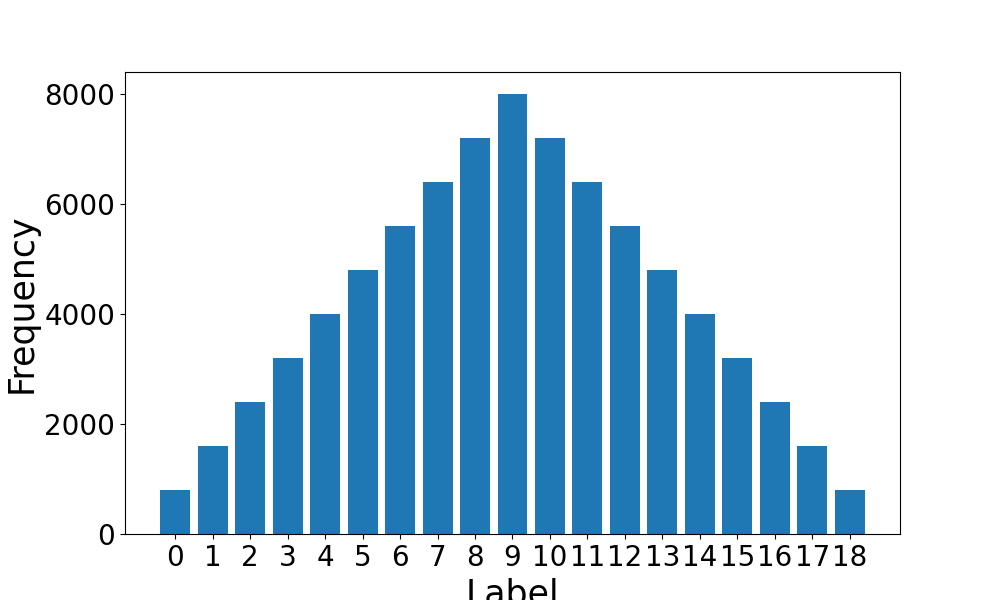
\includegraphics[width=\columnwidth, keepaspectratio]{../Y_dist_many.png}
    \caption{Distribution of labels in a dataset of 80,000 samples.}\label{fig:manysamples}
\end{figure}

\begin{figure}
    \centering
    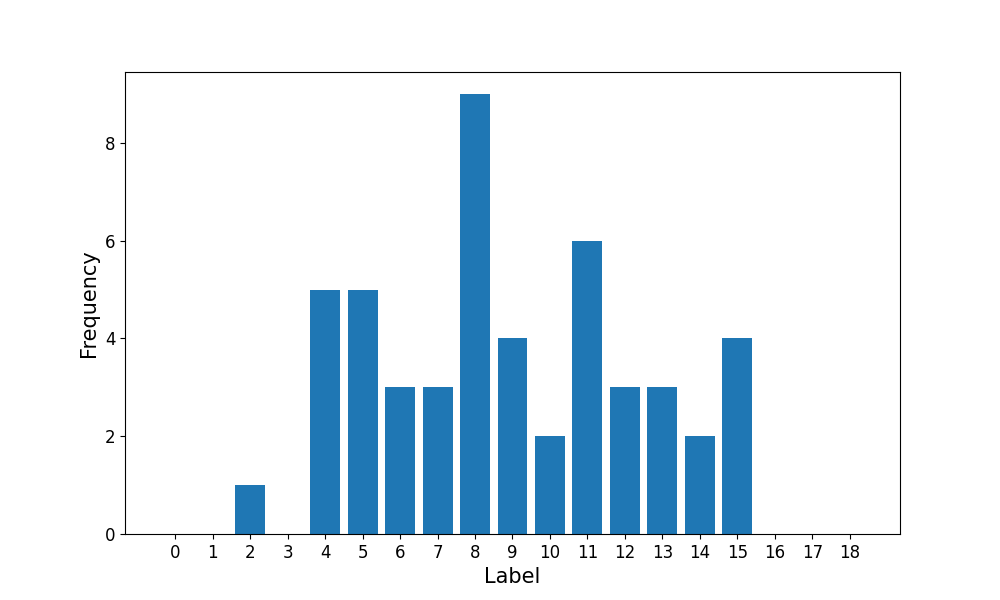
\includegraphics[width=\columnwidth, keepaspectratio]{../Y_dist_few.png}
    \caption{Distribution of labels in a dataset of 50 samples.}\label{fig:fewsamples}
\end{figure}

\section{Neural network pipeline}
\texttt{Tensorflow} was used to create the neural network architecture and \texttt{Optuna} was used to tune the hyperparameters for this architecture.

\subsection{Neural networks}
The neural network used for this project is a \texttt{Sequential} model, where each layer has exactly one input tensor and one output tensor. This is a feedforward neural network, where information passes through the layers in only one direction, starting at the input layer, through the hidden \texttt{Dense} layers, and exiting at the output layer. In the hidden layers, each neuron computes a weighted sum of its inputs, adds a bias, and then applies a non-linear activation function to generate the layer's output. The outputs of each \texttt{Dense} layer become the inputs of the following \texttt{Dense} layer. The final output layer, which in this project has as many neurons as there are classes, produces the probabilities of the digit pair adding up to be any of the numbers in the range 0--18.

For this project, the rectified linear unit (ReLU) activation function was used. This is because ReLU tends be computationally efficient and shows better convergence than sigmoid functions \citep{Zeiler2013relu}.

In order to train feed forward neural networks, a loss function is required. For this project, the loss function $\mathcal{L} (\theta, \hat{\theta})$ was the categorical cross-entropy loss function, which is used for multi-class classification problems. It is defined as
\begin{equation}
    \mathcal{L}(\theta, \hat{\theta}) = - \frac{1}{N}\sum^N_{i=1}\sum^C_{j=1} \theta_{ij} \log{\hat{\theta_{ij}}},
    \label{eq:loss}
\end{equation}
where $\theta_{ij}$ is the true value of the $i$th element belonging to the $j$th class and $\hat{\theta_{ij}}$ is the predicted value of that element. This function is used to calculate the loss during training with the backpropagation algorithm, which computes the gradients of the loss with respect to each weight by applying the chain rule. This allows the neural network to learn how to adjust its weights by optimising this function. The weights are adjusted using the Adam optimisation function in the following process:

\begin{enumerate}
    \item The model parameters $\theta$; learning rate $\alpha$; and Adam hyperparameters $\beta_1$, $\beta_2$, and $\epsilon$ are initialised.
    \item The gradient $g$ of the loss function $\mathcal{L}$ with respect to the model parameters $\theta$ are computed:
        \begin{equation}
            g^{(t)} = \nabla \mathcal{L}(\theta^{(t-1)})
        \end{equation}
    \item The first moment estimate $m$ is updated:
        \begin{equation}
            m^{(t)} = \beta_1 m^{(t-1)} + (1-\beta_1)g^{(t)}
        \end{equation}
    \item The second moment estimate $v$ is updated:
        \begin{equation}
            v^{(t)} = \beta_2 v^{(t-1)} + (1-\beta_2)[g^{(t)}]^2
        \end{equation}
    \item The biases for $m$ and $v$ are corrected:
        \begin{equation}
            \hat{m}^{(t)} = \frac{m^{(t)}}{1-\beta^t_1}, \qquad
            \hat{v}^{(t)} = \frac{v^{(t)}}{1-\beta^t_2}
        \end{equation}
    \item The adaptive learning rate $\alpha^{(t)}$ is updated:
        \begin{equation}
            \alpha^{(t)} = \frac{\alpha^{(t-1)}\sqrt{1-\beta^t_2}}{1-\beta^t_1}
        \end{equation}
    \item Finally, the model parameters $\theta^{(t)}$ are updated:
        \begin{equation}
            \theta^{(t)} = \theta^{(t-1)}\frac{\alpha^{(t)}\hat{m}^{(t)}}{\sqrt{\hat{v}^{(t)}} + \epsilon}
        \end{equation}
\end{enumerate}

\subsection{Hyperparameter Tuning}
For this project, 5 hyperparameters were tuned: the initial learning rate for the Adam optimiser, the dropout rate of the dropout layers, the L2 regularisation penalty, the number of layers, and the batch size carried over from each layer. In addition to this, batch normalisation was also used.

The Adam optimisation algorithm is a stochastic gradient descent method that is based on adaptive estimation of first-order and second-order moments \citep{kingma2017adammethodstochasticoptimization}. It was used as it is computationally efficient and well-suited to large-scale problems, as advised by Kingma and Ba \citep{kingma2017adammethodstochasticoptimization}. The inital learning rate $\alpha^{(0)}$ was tuned for the optimal rate of adaptative estimation. Too-large of a learning rate can lead to missing the minimum entirely, while too-small of a learning rate leads to computationally-inefficient code.

The dropout rate of the dropout layers was tuned so that the resulting neural network would not over-fit to the training data but also not forget what it was meant to be fitting during training \citep{Mehta_2019}. In \texttt{Tensorflow}, the \texttt{Dropout} layer randomly resets neurons to zero with a certain frequency. The rest of the neurons are scaled up such that the total sum over all inputs remain unchanged.

Regularisation is when a penalty is added to the loss function $\mathcal{L}$ in order to prevent overfitting \citep{Mehta_2019}. L2 regularisation, or ridge regression, adds the squared sum of the coefficients as the penalty term. Adding L2 regularisation to Eq.~\ref{eq:loss} results in the following equation:
\begin{equation}
    \mathcal{L}(\theta, \hat{\theta}, \alpha_{L2}, \mathrm{w}) = - \frac{1}{N}\sum^N_{i=1}\sum^C_{j=1} \theta_{ij} \log{\hat{\theta_{ij}}} + \alpha_{L2} ||\mathrm{w}||^2_2,
\end{equation}
where $\theta_{ij}$ and $\hat{\theta}_{ij}$ mean the same things, $\alpha_{L2}$ refers to the penalty parameter, and $||\mathrm{w}||^2_2$ is the L2 norm squared of the weight vector of the parameters.

L2 regularisation was preferred over L1 regularisation as its derivative is smooth and continuous and thus less computationally expensive.

The number of layers were tuned so that the neural network would neither overfit nor underfit. The range of the number of layers to tune was restricted so that neither too many layers were attempted, which would have required a lot of computational resources, nor too few, which would have failed to properly capture all relevant features of the dataset.

The batch size was also tuned to determine the number of training samples used in one epoch of training. Larger batch sizes represent more of the total dataset, which helps in computing more accurate estimations of the gradient, but are more computationally expensive and also might lead to overfitting. Smaller batch sizes tend to introduce noise, but are faster to compute.

The number of neurons in each layer was not a hyperparameter that was tuned using \texttt{Optuna}. Instead, the number of neurons were dependant upon the number of layers and constructed such that each successive layer has fewer neurons than the last. This can be represented as:

\begin{equation}
    N_k = 2^{N-1-k} \times 64, \quad\mathrm{for}\ k=0, 1, 2, \dots, N-1,
\end{equation}
where $N_k$ is the number of neurons in layer $k$.

Batch normalisation is a regularisation scheme that causes the inputs to be centered about zero with respect to the bias \citep{Mehta_2019}. This prevents neuron saturation and gradients vanishing, improving the learning speed. This was implemented by adding \texttt{BatchNormalization} layers which standardised the inputs by the mean and variance of the mini-batch.

The results of the \texttt{Optuna} hyperparameter tuning is shown in Table~\ref{tab:nn_hyperparameter}, which contains the optimal hyperparameters. As the final architecture contains 6 hidden \texttt{Dense} layers, the number of neurons in each layer range from 2048 to 64, descending, as seen in Table~\ref{tab:neurons}. The architecture of the best-performing neural network is shown in Table~\ref{tab:nn_arch}.

\begin{table}[ht]
    \centering
    \begin{tabular}{c|c}
        Hyperparameter & Value\\
        \hline
        Adam initial learning rate $\alpha$ & 0.000236 (3 s.f.) \\
        Dropout rate & 0.104 (3 s.f.) \\
        L2 penalty parameter $\alpha_{L2}$ & 0.000189 (3 s.f.) \\
        Number of layers & 6 \\
        Batch size & 69 \\
    \end{tabular}
    \caption{Values of the hyperparameters of the best-performing neural network.}\label{tab:nn_hyperparameter}
\end{table}

\begin{table}[ht]
    \centering
    \begin{tabular}{c|c|c|c|c|c|c}
        &\multicolumn{6}{c}{\texttt{Dense} Layer} \\
        \cline{2-7}
         & 1 & 2 &3 &4 &5&6\\
        \hline
        Neurons & 2048 & 1024 & 512 & 256 & 128 & 64 \\
    \end{tabular}
    \caption{The number of neurons in each layer of the best-performing neural network.}\label{tab:neurons}
\end{table}

\begin{table}[ht]
    \centering
    \begin{tabular}{c|c|c}
        Layer & Type & Additional information\\
        \hline
        1 & Input layer & 28 $\times$ 56 input shape\\
        2 & \texttt{Dense} layer & 2048 neurons \\
        3 & \texttt{Dropout} layer & 0.104 dropout rate \\
        4 & \texttt{BatchNormalization} layer \\
        5 & \texttt{Dense} layer & 1024 neurons \\
        6 & \texttt{Dropout} layer & 0.104 dropout rate\\
        7 & \texttt{BatchNormalization} layer \\
        8 & \texttt{Dense} layer & 512 neurons \\
        9 & \texttt{Dropout} layer & 0.104 dropout rate\\
        10 & \texttt{BatchNormalization} layer \\
        11 & \texttt{Dense} layer & 256 neurons \\
        12 & \texttt{Dropout} layer & 0.104 dropout rate\\
        13 & \texttt{BatchNormalization} layer \\
        14 & \texttt{Dense} layer & 128 neurons \\
        15 & \texttt{Dropout} layer & 0.104 dropout rate\\
        16 & \texttt{BatchNormalization} layer \\
        17 & \texttt{Dense} layer & 64 neurons \\
        18 & \texttt{Dropout} layer & 0.104 dropout rate\\
        19 & \texttt{BatchNormalization} layer \\
        20 & Output layer & 19 neurons\\
    \end{tabular}
    \caption{The architecture of the best-performing neural network.}\label{tab:nn_arch}
\end{table}
\newpage
\subsection{Results}
The best-performing neural network was evaluated using \texttt{Tensorflow}'s \texttt{tf.keras.Model .evaluate} method. The results of this can be seen in Table~\ref{tab:nn_eval}.
\begin{table}[ht]
    \centering
    \begin{tabular}{c|c}
        Metrics & Value (3 s.f.)\\
        \hline
        Accuracy & 0.955 \\
    \end{tabular}
    \caption{The metrics of the best-performing neural network as calculated by \texttt{tf.keras. Model.evaluate}.}\label{tab:nn_eval}
\end{table}

The resulting confusion matrix is shown in Fig.~\ref{fig:nn_confusion}. The rows represent the true class label of each digit pair whilst the columns represent the predicted class labels from the neural network. Off-diagonal elements represent misclassifications.

\begin{figure}[ht]
    \centering
    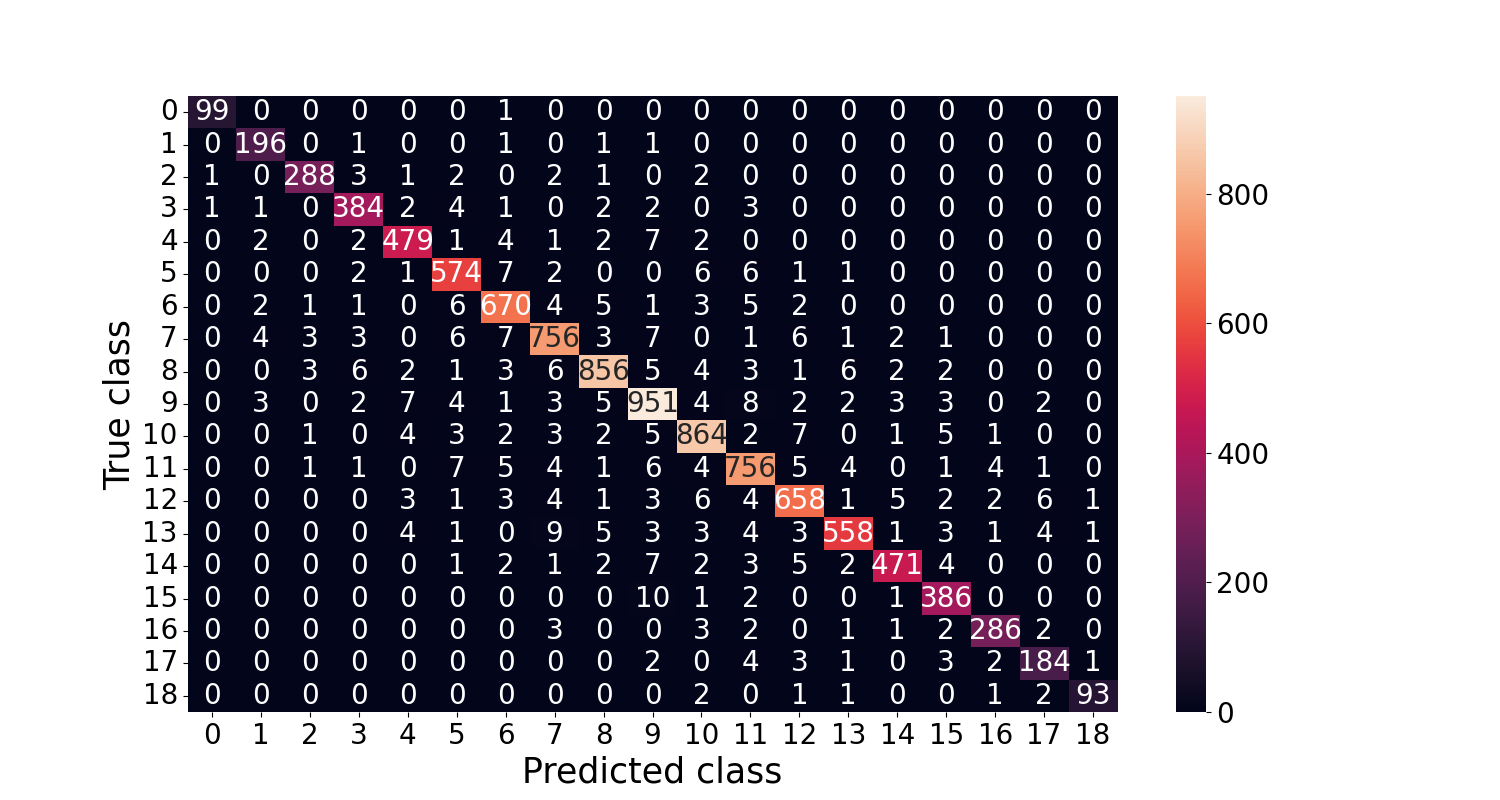
\includegraphics[width=\columnwidth, keepaspectratio]{../confusion_nn.png}
    \caption{Confusion matrix of the best-performing neural network. }\label{fig:nn_confusion}
\end{figure}

An example of the neural network in action can be seen in Fig.~\ref{fig:nn_predict}. The neural network's predictions are quite accurate, except for the first image, where the number '8' is quite deformed. It is likely that the neural network mistook it as a '7' instead, and then proceeded to correctly perform addition: $7+1=8$.

\begin{figure}[ht]
    \centering
    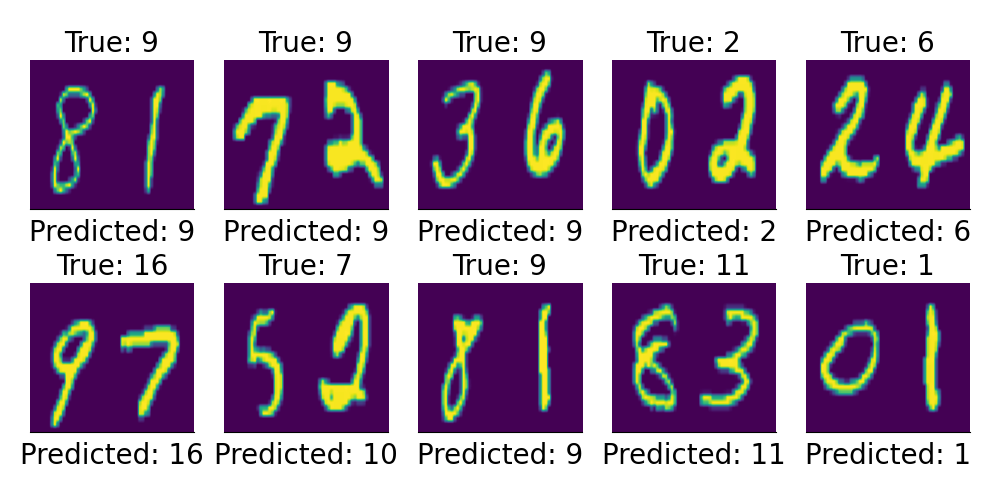
\includegraphics[width=\columnwidth, keepaspectratio]{../nn_predictions.png}
    \caption{Ten images of random digit pairs, their true labels, and the corresponding predictions given by the best-performing neural network.}\label{fig:nn_predict}
\end{figure}

\clearpage
\section{Other inference algorithms}
To explore this problem further, other inference algorithms were used, including SVMs, Random Forest classifiers, and AdaBoost classifiers.
\subsection{SVM}
SVM stands for Support Vector Machine, which is a supervised learning method used for classification in machine learning. SVMs find the optimal hyperplane for a linearly separable pattern.

The SVM classifier was implemented using \texttt{scikit-learn}'s \texttt{sklearn.svm.SVC} class. \texttt{Optuna} was used to tune the $\gamma$, $c$, and polynomial degree hyperparameters. The polynomial kernel trick produced the best-performing SVM classifier during initial tuning, thus that kernel trick was the one used for further tuning.

During training, it was found that the best-performing SVM was one with a large number of training samples. However, SVMs have an order complexity around $\mathcal{O}(N^2)$ \citep{Chang2007} and it is for this reason \texttt{Optuna} hyperparameter tuning was limited to 10,000 samples and training was limited to 64,000 samples.

The hyperparameters of the best-performing SVM can be found in Table~\ref{tab:svm_hyperparameter}. This was evaluated using \texttt{scikit-learn}'s \texttt{sklearn.metrics.accuracy\_score} and \texttt{classification \_report} methods, resulting in Table~\ref{tab:svm_eval}. Precision refers to the positive predictive value and is the fraction of predicted positive results that are true. Recall refers to the fraction of true positive results that are predicted to be true. The F-score is calculated from the precision and recall, as seen in Eq.~\ref{eq:fscore} and ranges from 0 to 1. The higher the F-score, the better. The resulting confusion matrix can be seen in Fig.~\ref{fig:svm_confusion}.

\begin{equation}
    F = 2\cdot\frac{\mathrm{precision}\cdot \mathrm{recall}}{\mathrm{precision} + \mathrm{recall}}\label{eq:fscore}
\end{equation}

\begin{table}[ht]
    \centering
    \begin{tabular}{c|c}
        Hyperparameter & Value\\
        \hline
        Kernel & Polynomial \\
        Degree & 3 \\
        Gamma ($\gamma$) & 21.8 (3 s.f.) \\
        $C$ & 1.61 (3 s.f.)\\
    \end{tabular}
    \caption{Values of the hyperparameters of the best-performing SVM.}\label{tab:svm_hyperparameter}
\end{table}

\begin{table}[ht]
    \centering
    \begin{tabular}{c|c|c|c|c}
        Class & Precision (2 s.f.) & Recall (2 s.f.)& F1-Score (2 s.f.)& Support \\
        \hline
        0  & 0.86 & 0.96 & 0.91 & 160 \\
        1  & 0.89 & 0.99 & 0.93 & 320 \\
        2  & 0.87 & 0.89 & 0.88 & 480 \\
        3  & 0.85 & 0.87 & 0.86 & 640 \\
        4  & 0.86 & 0.86 & 0.86 & 800 \\
        5  & 0.82 & 0.85 & 0.83 & 960 \\
        6  & 0.82 & 0.82 & 0.82 & 1120 \\
        7  & 0.80 & 0.80 & 0.80 & 1280 \\
        8  & 0.77 & 0.79 & 0.78 & 1440 \\
        9  & 0.80 & 0.81 & 0.80 & 1600 \\
        10 & 0.77 & 0.78 & 0.78 & 1440 \\
        11 & 0.76 & 0.72 & 0.74 & 1280 \\
        12 & 0.79 & 0.78 & 0.79 & 1120 \\
        13 & 0.79 & 0.78 & 0.78 & 960 \\
        14 & 0.81 & 0.77 & 0.79 & 800 \\
        15 & 0.82 & 0.76 & 0.79 & 640 \\
        16 & 0.81 & 0.79 & 0.80 & 480 \\
        17 & 0.81 & 0.76 & 0.78 & 320 \\
        18 & 0.81 & 0.88 & 0.84 & 160 \\
        % \hline
        % Macro average & 0.82 & 0.82 & 0.82 & 16000 \\
        % Weighed average & 0.80 & 0.80 & 0.80 & 16000 \\
        \hline
        Total accuracy (2 s.f.) &\multicolumn{3}{c|}{0.80} & 16000 \\

    \end{tabular}
    \caption{Classification report of the best-performing SVM along with the total accuracy of the SVM's performance on the test dataset.}\label{tab:svm_eval}
\end{table}

\begin{figure}[h]
    \centering
    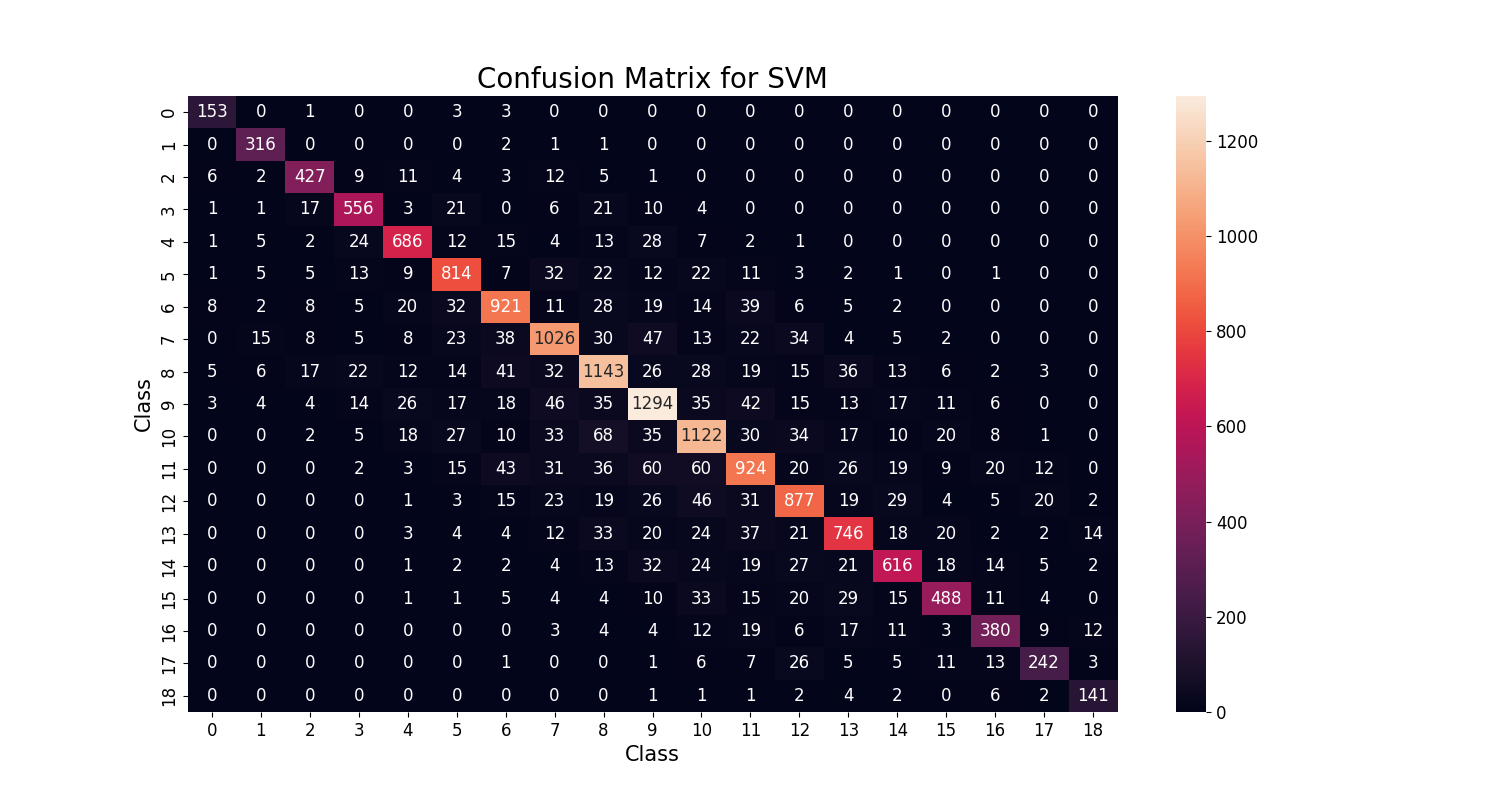
\includegraphics[width=\columnwidth, keepaspectratio]{../confusion_SVM.png}
    \caption{Confusion matrix of the best-performing SVM.}\label{fig:svm_confusion}
\end{figure}

\clearpage
\subsection{Random forest}
Random forest classifiers are a type of ensemble classifier, where multiple decision trees are used in aggregate in order to calculate predicted labels. Hyperparameter tuning and training for the best-performing random forest was much quicker than for SVMs and offered similar accuracies. This is because the time complexity for training random forest is on the order $\mathcal{O}(N M D \log({N}) )$, where $N$ is the number of samples, $M$ the number of classes, and $D$ the number of decision trees \citep{Zheng2021}.

Hyperparameter tuning used for their maximum depth, the number of allowed decision trees, the criterion to measure the quality of a split, and the method to calculate the maximum number of features to consider when looking for the best split. The optimal hyperparameters can be found in Table~\ref{tab:rf_hyperparameter}.

\begin{table}[ht]
    \centering
    \begin{tabular}{c|c}
        Hyperparameter & Value\\
        \hline
        Depth & 591 \\
        Trees & 249 \\
        Criterion & gini \\
        Maximum features & $\sqrt{19}$\\
    \end{tabular}
    \caption{Values of the hyperparameters of the best-performing random forest.}\label{tab:rf_hyperparameter}
\end{table}

'Gini' refers to the Gini impurity \citep{Breiman2017-zt}, where the impurity of a node is calculated through Eq.~\ref{eq:gini}

\begin{equation}
    \mathrm{gini} = 1- \sum_i p^2_i\label{eq:gini},
\end{equation}

where $p_i$ refers to the probability of class $i$. When the impurity is zero, all elements within a node are of the same class.

The results of the best-performing random forest classifier's evaluation can be found in Table~\ref{tab:rf_eval}. The random forest's confusion matrix is shown in Fig.~\ref{fig:rf_confusion}.

\begin{table}[t]
    \centering
    \begin{tabular}{c|c|c|c|c}
        Class & Precision (2 s.f.) & Recall (2 s.f.)& F1-Score (2 s.f.)& Support \\
        \hline
        0  & 0.90 & 0.97 & 0.94 & 160 \\
        1  & 0.88 & 0.97 & 0.92 & 320 \\
        2  & 0.88 & 0.86 & 0.87 & 480 \\
        3  & 0.87 & 0.84 & 0.86 & 640 \\
        4  & 0.86 & 0.81 & 0.83 & 800 \\
        5  & 0.85 & 0.80 & 0.83 & 960 \\
        6  & 0.82 & 0.81 & 0.81 & 1120 \\
        7  & 0.84 & 0.79 & 0.81 & 1280 \\
        8  & 0.73 & 0.80 & 0.77 & 1440 \\
        9  & 0.73 & 0.84 & 0.78 & 1600 \\
        10 & 0.75 & 0.78 & 0.76 & 1440 \\
        11 & 0.71 & 0.77 & 0.74 & 1280 \\
        12 & 0.70 & 0.79 & 0.74 & 1120 \\
        13 & 0.78 & 0.76 & 0.77 & 960 \\
        14 & 0.83 & 0.65 & 0.73 & 800 \\
        15 & 0.88 & 0.73 & 0.80 & 640 \\
        16 & 0.79 & 0.66 & 0.72 & 480 \\
        17 & 0.82 & 0.60 & 0.69 & 320 \\
        18 & 0.87 & 0.63 & 0.73 & 160 \\
        % \hline
        % Macro average & 0.82 & 0.78 & 0.79 & 16000 \\
        % Weighed average & 0.79 & 0.79 & 0.79 & 16000 \\
        \hline
        Total accuracy (2 s.f.) &\multicolumn{3}{c|}{0.79} & 16000 \\

    \end{tabular}
    \caption{Classification report of the best-performing random forest along with the total accuracy of the random forest's performance on the test dataset.}\label{tab:rf_eval}
\end{table}

\begin{figure}[htb]
    \centering
    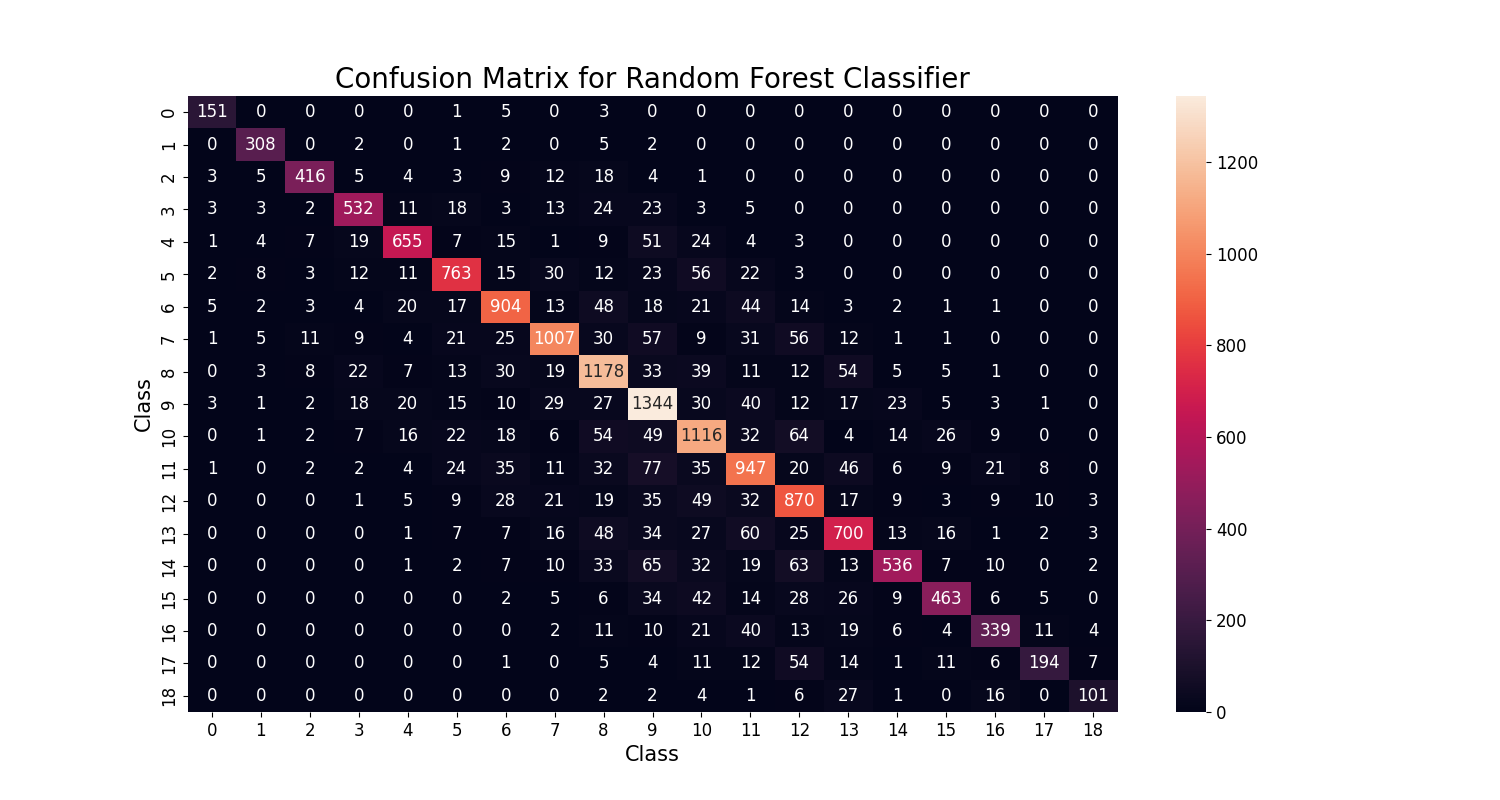
\includegraphics[width=\columnwidth, keepaspectratio]{../confusion_Random Forest Classifier.png}
    \caption{Confusion matrix of the best-performing random forest.}\label{fig:rf_confusion}
\end{figure}

\clearpage
\subsection{AdaBoost}
AdaBoost classifiers are another type of ensemble classifier, which trains multiple weak classifiers subsets of the training data. In each iteration, the AdaBoost algorithm assigns higher weights and thus focuses more on misclassified samples from previous iterations. This allows the weak classifiers to improve their performance by spending the majority of their time training on the previously misclassified samples. 

The AdaBoost classifier used in this project used the decision stump classifier as its weak classifier. Hyperparameter tuning was performed on the number of decision trees used. The number of hyperparameters tuned was deliberately limited as tuning and training of the AdaBoost classifier took very long amounts of time and did not produce very accurate classifiers. This is to be expected as decision stumps do not perform very well on multi-class datasets. However, this classifier still produced an accuracy of 14\%, which is still better than random guessing, which has an accuracy of 5.2\% for a 19-feature dataset.

The optimal hyperparameters can be found in Table~\ref{tab:ab_hyperparameter}. The result of the AdaBoost classifier evaluation can be found in Table~\ref{tab:ab_eval} and the resulting confusion matrix is shown in Fig.~\ref{fig:ab_confusion}.

\begin{table}[ht]
    \centering
    \begin{tabular}{c|c}
        Hyperparameter & Value\\
        \hline
        Stumps & 53 \\
    \end{tabular}
    \caption{Values of the hyperparameters of the best-performing AdaBoost.}\label{tab:ab_hyperparameter}
\end{table}

\begin{table}[ht]
    \centering
    \begin{tabular}{c|c|c|c|c}
        Class & Precision (2 s.f.) & Recall (2 s.f.)& F1-Score (2 s.f.)& Support \\
        \hline
        0  & 0.90 & 0.97 & 0.94 & 160 \\
        1  & 0.88 & 0.97 & 0.92 & 320 \\
        2  & 0.88 & 0.86 & 0.87 & 480 \\
        3  & 0.87 & 0.84 & 0.86 & 640 \\
        4  & 0.86 & 0.81 & 0.83 & 800 \\
        5  & 0.85 & 0.80 & 0.83 & 960 \\
        6  & 0.82 & 0.81 & 0.81 & 1120 \\
        7  & 0.84 & 0.79 & 0.81 & 1280 \\
        8  & 0.73 & 0.80 & 0.77 & 1440 \\
        9  & 0.73 & 0.84 & 0.78 & 1600 \\
        10 & 0.75 & 0.78 & 0.76 & 1440 \\
        11 & 0.71 & 0.77 & 0.74 & 1280 \\
        12 & 0.70 & 0.79 & 0.74 & 1120 \\
        13 & 0.78 & 0.76 & 0.77 & 960 \\
        14 & 0.83 & 0.65 & 0.73 & 800 \\
        15 & 0.88 & 0.73 & 0.80 & 640 \\
        16 & 0.79 & 0.66 & 0.72 & 480 \\
        17 & 0.82 & 0.60 & 0.69 & 320 \\
        18 & 0.87 & 0.63 & 0.73 & 160 \\
        % \hline
        % Macro average & 0.82 & 0.78 & 0.79 & 16000 \\
        % Weighed average & 0.79 & 0.79 & 0.79 & 16000 \\
        \hline
        Total accuracy (2 s.f.) &\multicolumn{3}{c|}{0.79} & 16000 \\

    \end{tabular}
    \caption{Classification report of the best-performing AdaBoost along with the total accuracy of the AdaBoost's performance on the test dataset.}\label{tab:ab_eval}
\end{table}

\begin{figure}[htb]
    \centering
    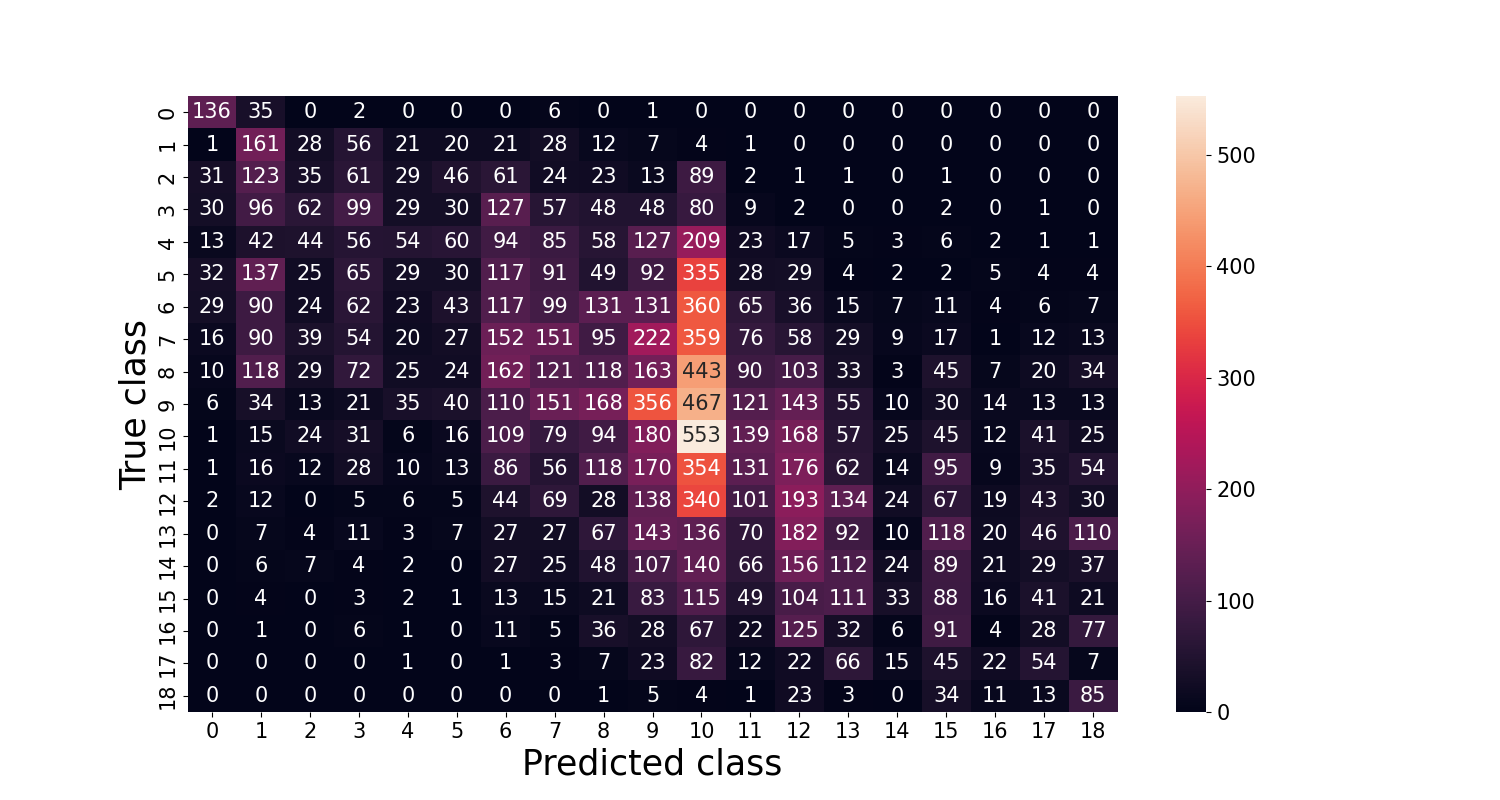
\includegraphics[width=\columnwidth, keepaspectratio]{../confusion_AdaBoost Classifier.png}
    \caption{Confusion matrix of the best-performing AdaBoost classifier.}\label{fig:ab_confusion}
\end{figure}

\section{Weak linear classifiers}
To explore this dataset further, the results of a single linear regression classifier trained on the whole image of the digit pair was compared to that of a linear regression classifier that was fitted to each digit of the pair sequentially. That is to say, the first classifier was trained on digit pairs, while the second was on trained on single digits.

An example of the resulting classifier probabilities is shown in Figures \ref{fig:class_prob} and \ref{fig:class_prob_bar}. The result is that the single classifier naturally has probabilities for label classes ranging from 0-18, whilst the sequential classifier's probability must be manually calculated, as it natively has probabilities for label classes ranging from 0-9. This calculation is trivial, as the digits of each pair are independent of each other and thus their probabilities can be directly multiplied.

The accuracy is also compared in Fig.~\ref{fig:class_compare}. As expected, the sequential classifier is more accurate by the single classifier as it is simply trained on single digit recognition and the labels are combined after the fact to produce the final labels. In comparison, the single linear regression classifier has the much harder task of both recognising the digit pair and performing addition.

For both classifiers, the most significant jump in accuracy is when the number of samples go from 50 to 100, as there are 100 possible permutations of digit pairs. After that, the accuracy still increases, but there is not as great of an improvement as before. The accuracies for both the single and sequential linear regression classifier can be found in Table~\ref{tab:lin_metric}.

\begin{figure}[htb]
    \centering
    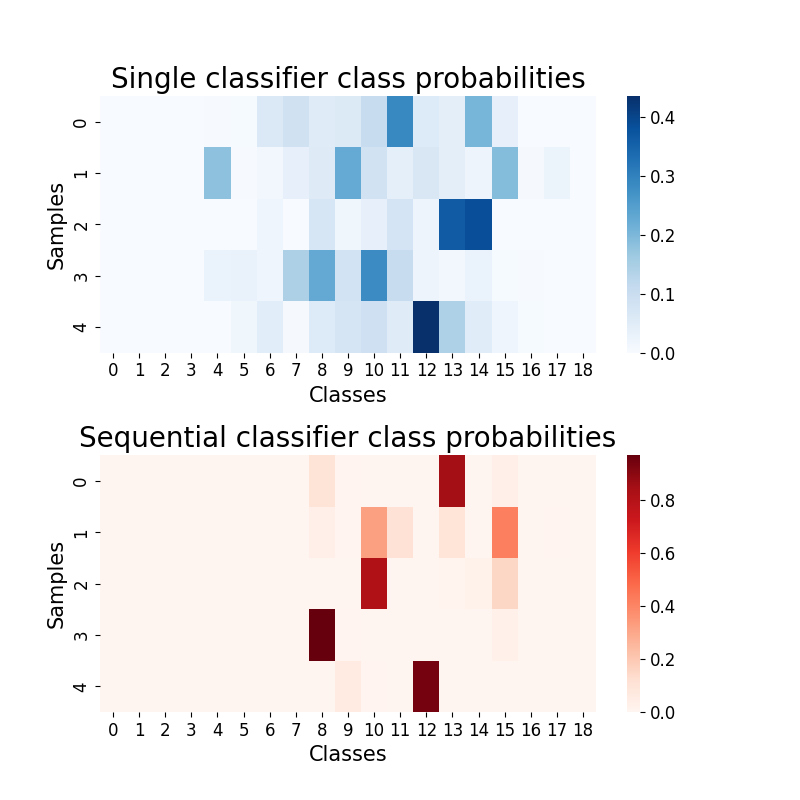
\includegraphics[width=\columnwidth, keepaspectratio]{../classifier_heatmap.png}
    \caption{Heatmaps of classifier probabilites for a single classifier (top) and a sequentially applied classifier (bottom). Shown are the first five class probabilities for linear regression classifiers trained on 10,000 samples.}\label{fig:class_prob}
\end{figure}

\begin{figure}[htb]
    \centering
    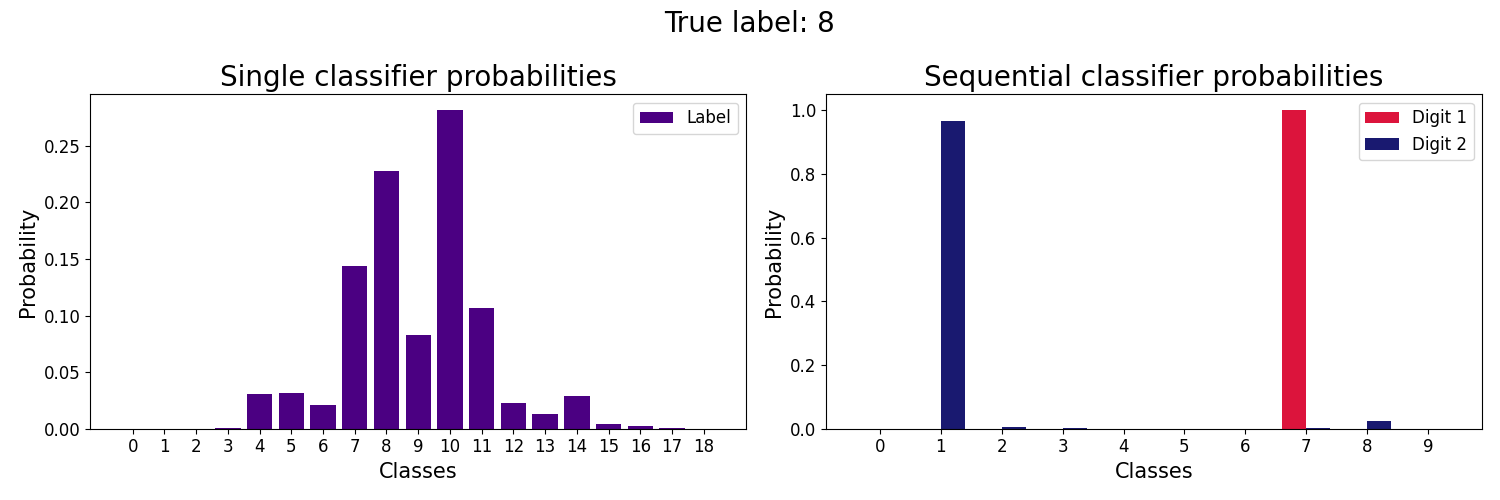
\includegraphics[width=\columnwidth, keepaspectratio]{../classifer_barplot.png}
    \caption{Barplot of classifier probabilites for a single classifier (left) and a sequentially applied classifier (right). Shown specifically are the probability distributions of sample 3 from Fig.~\ref{fig:class_prob}.}\label{fig:class_prob_bar}
\end{figure}

\begin{figure}[htb]
    \centering
    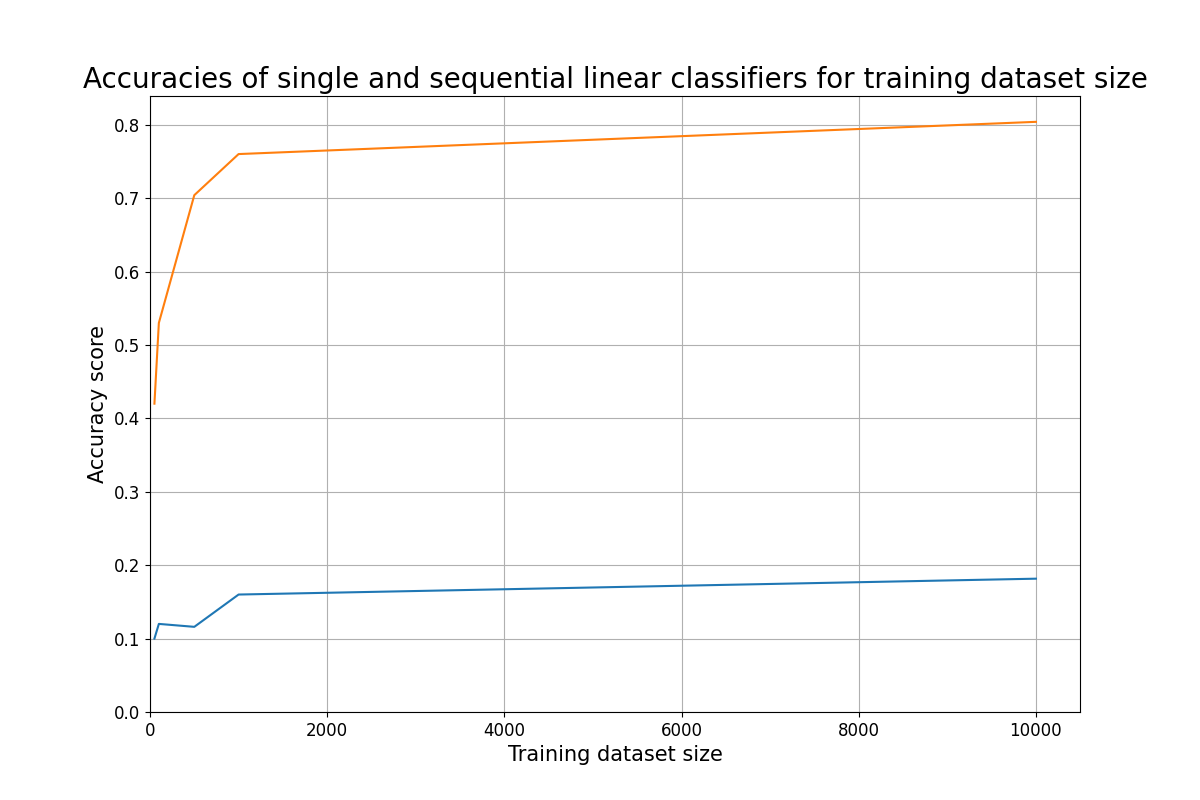
\includegraphics[width=\columnwidth, keepaspectratio]{../classifier_compare.png}
    \caption{Accuracy comparison between single and sequential linear regression classifiers as dependant on sample size.}\label{fig:class_compare}
\end{figure}

\begin{table}[ht]
    \centering
    \begin{tabular}{c|c|c|c|c|c}
        & \multicolumn{5}{c}{Sample sizes} \\
        \cline{2-6}
        Accuracy& 50 & 100 & 500 & 1000 & 10000\\
        \hline
        Single classifier (2 s.f.)& 0.08 & 0.10 & 0.11 &0.14 &0.18\\
        Sequential classifier (2 s.f.)& 0.36 & 0.71 &0.73 &0.75& 0.82\\
    \end{tabular}
    \caption{Accuracies of the single and sequential linear regression classifiers as sample sizes increase.}\label{tab:lin_metric}
\end{table}
\clearpage
\section{t-SNE distributions in neural networks}
The t-SNE distributions of the raw input data and the embedding layer of the best-performing neural network were obtained and optimised for perplexity. t-SNE refers to stochastic nieghbour embedding and is appropriate for visualisation of high-dimensional datasets \citep{JMLR:v9:vandermaaten08a}. What occurs is unsupervised learning where each datapoint is given a location in 2D space, similarities between data points are converted to joint probabilities and the Kullback-Lieber divergence between joint probabilities of the low-dimensional embedding and the high-dimensional data are minimised.

Perplexity is a hyperparameter for t-SNE and it relates to the number of nearest neighbours allowed. The higher the perplexity, the greater the variance. Perplexity was first optimised by eye in Fig.~\ref{fig:tsne} and then by silhouette score, which is a metric used to measure the quality of clustering results. The best-performing t-SNE according to silhouette score is shown in Fig.~\ref{fig:best_tsne}.

In comparison to the t-SNE representation of the input data to the embedding layer, the data from the embedding layer is much easier to separate into the requisite classes than the data from the input layer. Even with high perplexity, the t-SNE distribution representation of the input layer appears mostly random with little structure. This is expected as there is high dimensionality in the input data and related data points may not be grouped together. This is highly likely, as the dataset was generated randomly. In contrast, the embedding layer of the neural network has similar inputs already mapped closer together and is more structured. Essentially, the neural network has already done the work of grouping similar data points together.

\begin{figure}[htb]
    \centering
    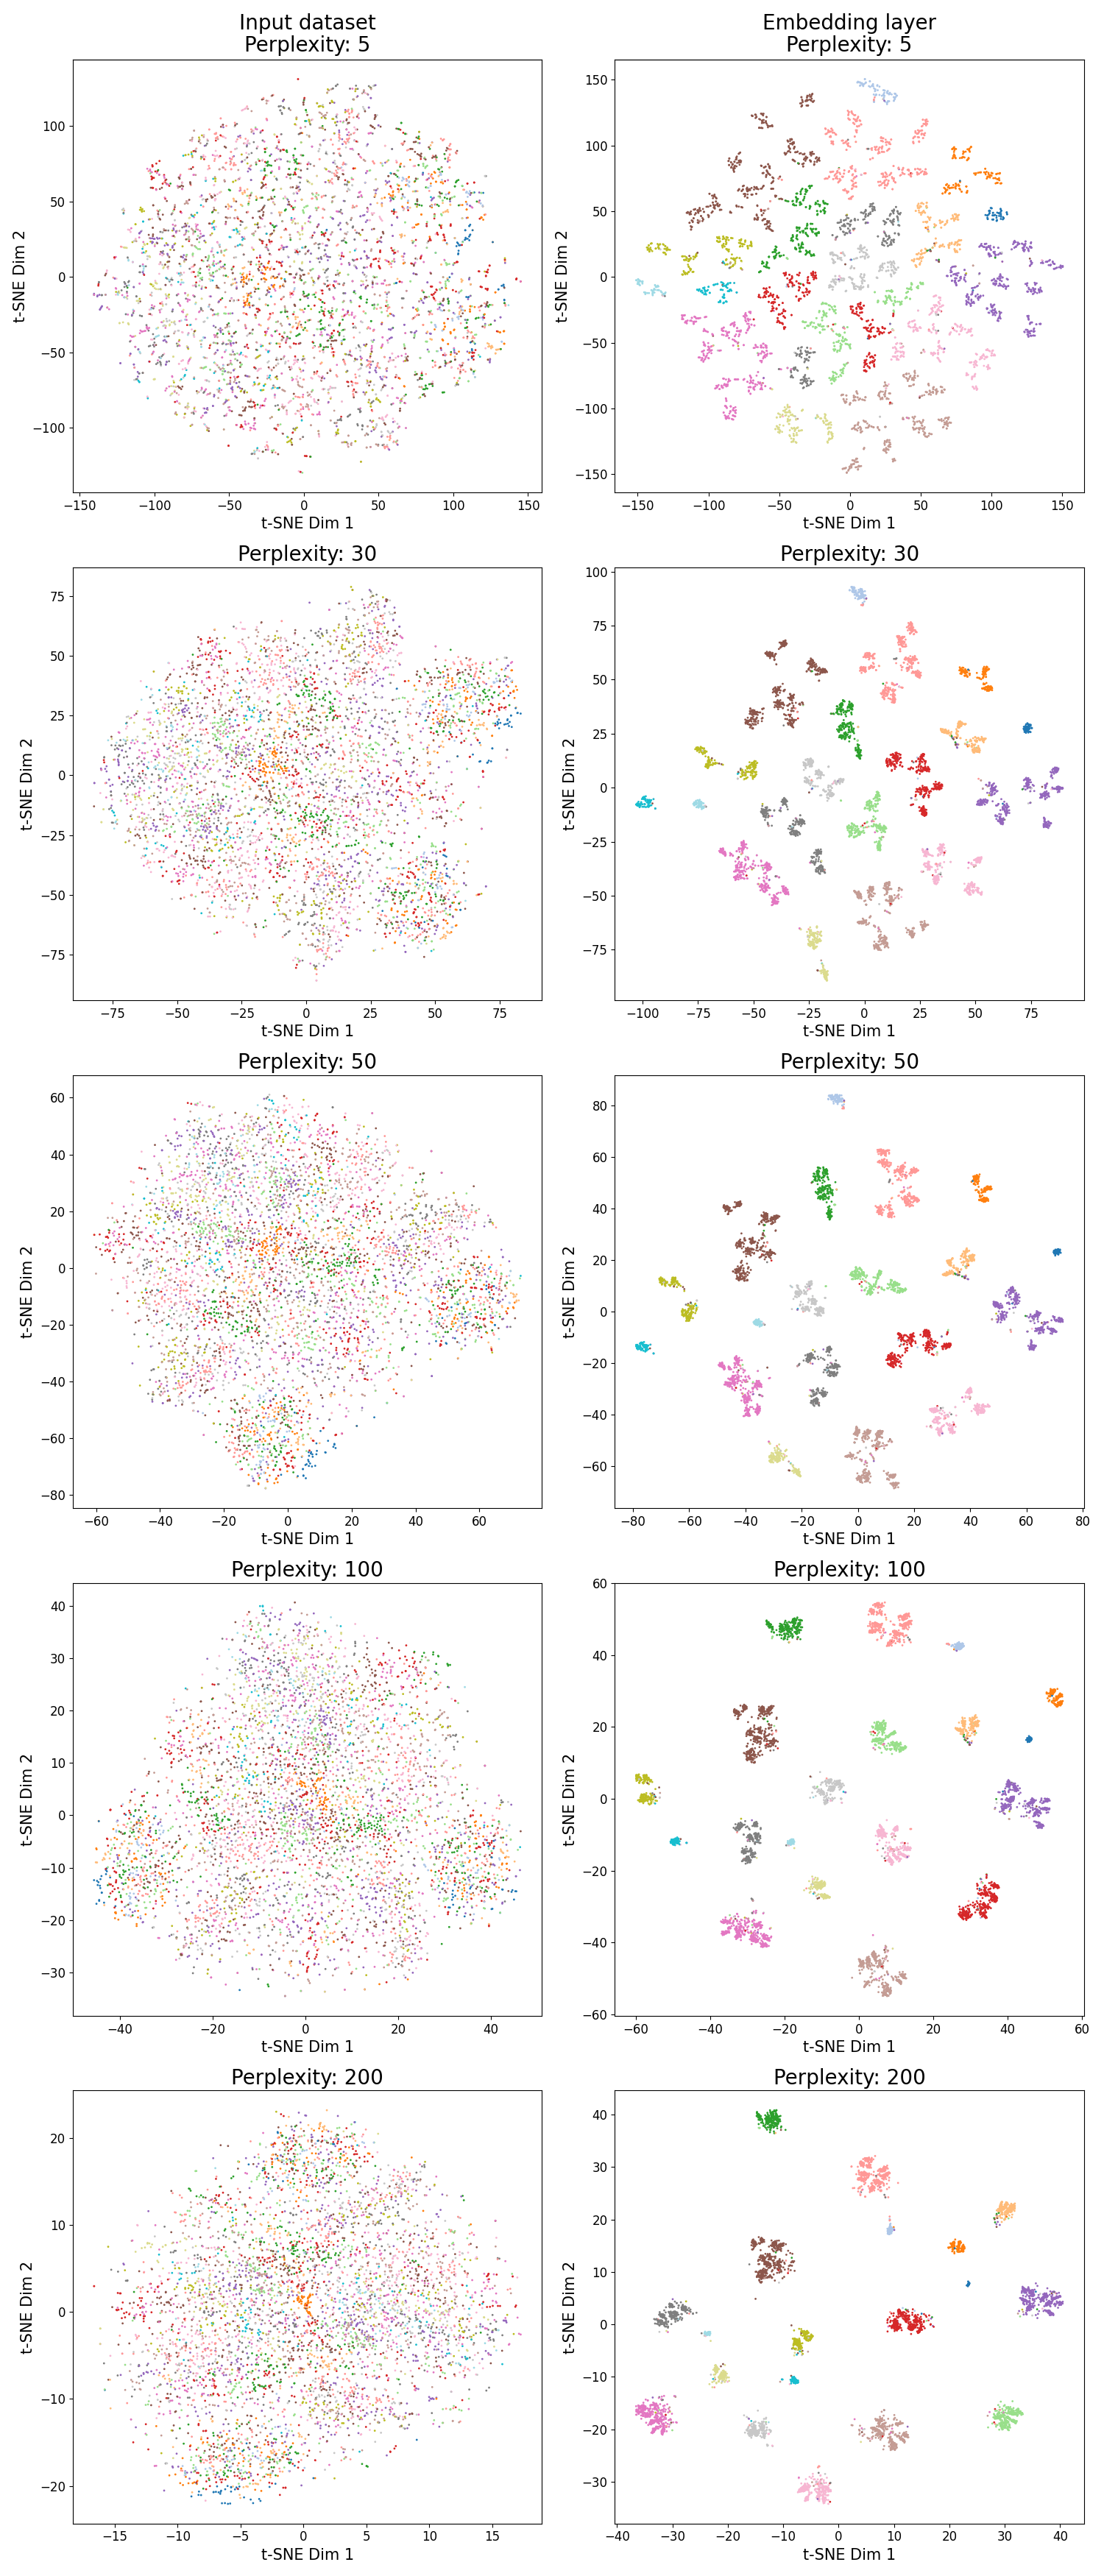
\includegraphics[width=\columnwidth, keepaspectratio]{../tsne.png}
    \caption{t-SNE distribution study as a function of complexity over the raw data and embedding layer of the best-performing neural network.}\label{fig:tsne}
\end{figure}

\begin{figure}[htb]
    \centering
    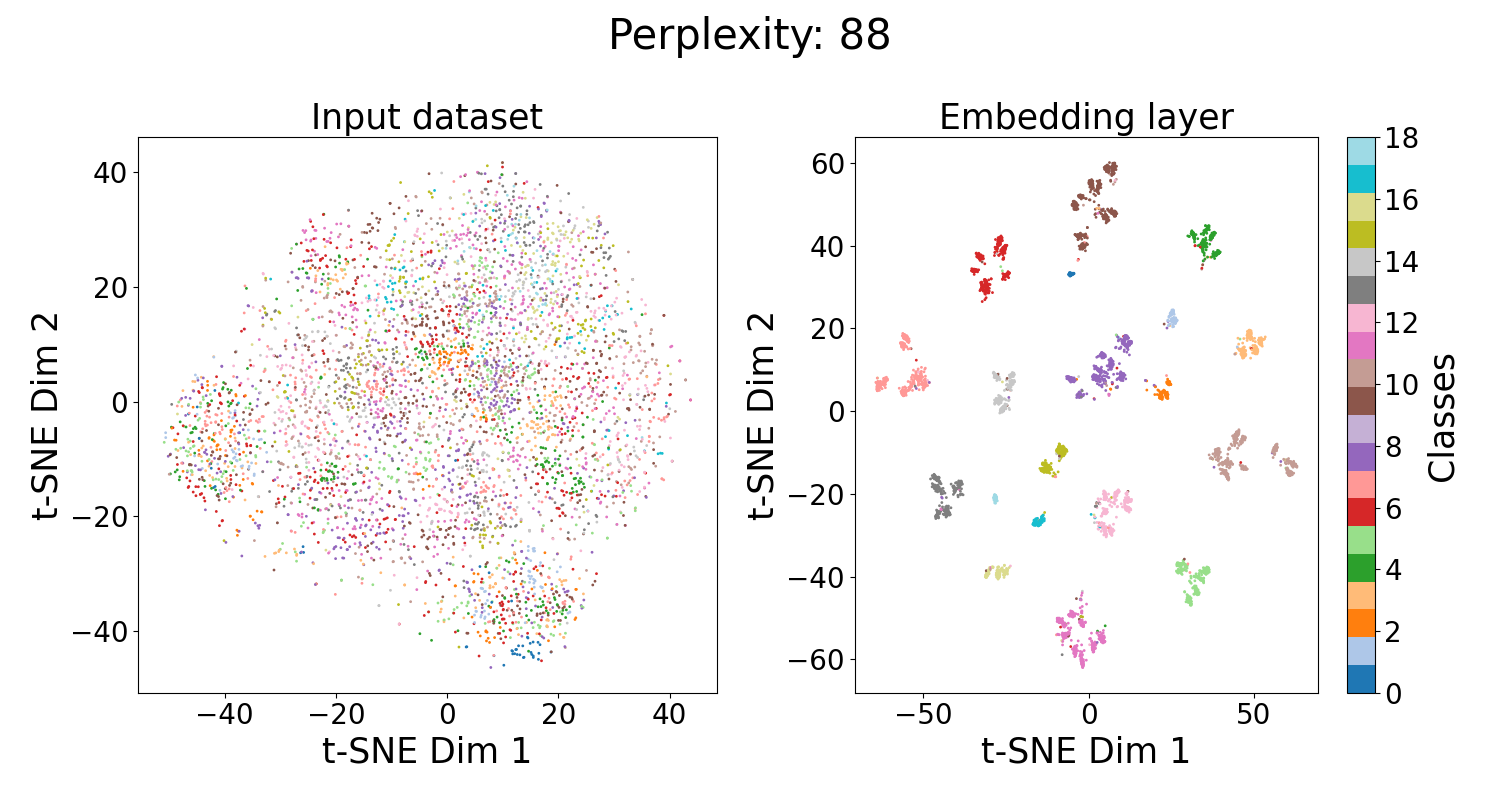
\includegraphics[width=\columnwidth, keepaspectratio]{../best_tsne.png}
    \caption{Best t-SNE distribution of the input data and embedding layer of the best-performing neural network, optimised over perplexity.}\label{fig:best_tsne}
\end{figure}
\clearpage
\section{Summary}
An inference pipeline for a neural network to recognise and add together MNIST digit pairs has been built with \texttt{Tensorflow}, hyperparameter tuned with \texttt{Optuna}, and trained to an accuracy of 95\%. Additionally, other inference algorithms have been explored, including SVMs, random forest classifiers, and AdaBoost classifiers, with respective accuracies of 80\%, 79\%, and 14\%. 

Linear regression classifiers have also been trained on the dataset, varying the number of samples. It was found that the greatest increase in accuracy comes from when the number of samples is enough to encompass all digit pair permutations.

Additionally, the t-SNE distribution of the input data and embedding layer of the best-performing neural network was produced with an optimal perplexity of 88. It was shown that the embedding layer is inherently more structured than the input data.
\clearpage
\bibliographystyle{vancouver}
\bibliography{bibliography}
\appendix
\section{Use of auto-generation tools}
Auto-generation tools were used to help setup \texttt{Tensorflow} on a WSL2 environment, parsing error messages throughout the project, and to help format this \LaTeX\ report.

Auto-generation tools were also used for code prototyping in plotting the results for task 4. Auto-generation tools were not used for code generation elsewhere.
\end{document}
